\documentclass[12pt,a4paper]{report}
\usepackage{amsmath}
\usepackage{amsfonts}
\usepackage{amssymb}
\usepackage{lmodern}
\usepackage[utf8x]{inputenc}
\usepackage[english]{babel}
\usepackage{ucs}
\usepackage{icomma}
\usepackage{siunitx}
\usepackage{subfiles}
\usepackage[hyphens]{url}
\usepackage[numbib,nottoc]{tocbibind}
\usepackage{mathtools}
\DeclarePairedDelimiter{\abs}{\lvert}{\rvert}
\DeclarePairedDelimiter{\norm}{\lVert}{\rVert}
\usepackage[bookmarks,hidelinks]{hyperref}
\usepackage{graphicx}
\usepackage{caption}
\usepackage{subfiles}
\usepackage{subfigure}
\usepackage{listings}
\usepackage{float}
\usepackage{booktabs}
\usepackage{titling}
\graphicspath{{../fig/}{./fig/}}
\renewcommand{\baselinestretch}{1.5}
\lstset{
  language=Matlab,
  keywordstyle=\bfseries\ttfamily\color[rgb]{0,0,1},
  identifierstyle=\ttfamily,
  commentstyle=\color[rgb]{0.133,0.545,0.133},
  stringstyle=\ttfamily\color[rgb]{0.627,0.126,0.941},
  showstringspaces=false,
  basicstyle=\small,
  numberstyle=\footnotesize,
  numbers=left,
  stepnumber=5,
  numberfirstline=true,
  breaklines=true,
  breakatwhitespace=false,
  frame=single
} 
\begin{document}
\title{Simulating mixing particles}
\author{Daniel O. Fejerskov, Mikkel S. Andersen Bennetsen,\\ Nathan H. Barr}
\maketitle
\tableofcontents

\chapter{Introduction}
In this report, we will simulate a system consisting of two different kinds of particles. In order to facilitate the presentation of the actual simulation itself, the first part of this report will be largely theoretical in nature. Here, we will describe the physical nature of the process that takes place when different kinds of particles interact and mix. The simulation itself is a Monte Carlo simulation, or more specifically the Metropolis algorithm. As this method of simulation was introduced in an earlier report in this course, we will not describe it in great detail, and only where it has relevance to the simulation itself. The second part of the report presents the method of simulation, as well as the results of it.

\chapter{Theory of Mixing}
In this section, we introduce the more important physical terms used in the report, and their relevance to the system we simulate. The goal of this report is to be able to make observations regarding the way the two types of particles interact. Specifically, a focal point of the report is to be able to show a phase diagram of their mixture. Further, we will be able to calculate, among other things the pressure of the system. This is done by determining the heat capacity of the system. From this we can calculate the entropy of the system, as a function of temperature. This result, in turn, we can use to calculate the Gibbs free energy of the system. This finally allows us to determine the pressure of the system.

\section{Heat Capacity and Entropy}
To calculate the heat capacity, we use the fluctuation function:

\begin{equation}\label{HeatC}
C_V = \left( \frac{\partial \langle E \rangle}{\partial T} \right)_{V,N}
\end{equation}
Here, the energy is simply an ensemble average. The point of calculating the heat capacity of our system is to be able to calculate the entropy. The calculation is naturally not straightforward in a simulation, but the general way of undertaking the operation is to realise that the heat capacity is related to the entropy by:
\begin{equation}
\frac{C_V}{T} = \left( \frac{\partial S}{\partial T}\right)_V
\end{equation}
In turn, this means that:

\begin{equation}
S = \int^{T_f}_{T_i} \frac{C_V}{T}\ dT
\end{equation}
Following this, we shall perform a thermodynamic integration of our result. This essentially means that we integrate at several different temperatures, in order to obtain the entropy of the system, as written above. In the next section, we summarise why this result is useful for calculating the Gibbs free energy and the pressure.

\subfile{gibbs.tex}




\chapter{Simulation}
In this chapter will introduce our simulations and results.

\section{Calculating Entropy}
As seen, entropy can be calculated by an integral, but before that can be used, we need an initial condition. The following is how we have calculated the initial condition where the temperature is equal to $\infty$. When our temperature approaches $\infty$, all states become equally probable. The multiplicity can be calculated as:

\begin{align}
\Omega=&\binom{N_A+N_B}{N_A}\binom{L^2}{N_A+N_B}, \;\; N_A+N_B\neq 0\\
=&\left(\frac{(N_A+N_B)!}{N_A!(N_A+N_B-N_A)!}\right) \left(\frac{L^2!}{(N_A+N_B)!(L^2-N_A+N_B)!}\right)
\end{align}
The entropy can be calculated as:

\begin{align}
S =& k_b \ln \left( \frac{(N_A+N_B)!}{N_A!(N_A+N_B-N_A)!}\right) \left( \frac{L^2!}{(N_A+N_B)!(L^2-N_A+N_B)!}\right)\\
=& k_b \left( \ln(m!)-\ln(N_A!)-\ln((m-N_A)!)+\ln(L^2!)-\ln(m!)- \ln((L^2-m)!) \right)\\
\approx& k_b [ m\ln(m)-m -((N_A\ln(N_A)-N_A)) - ((m-N_A)\ln(m-N_A)-(m-N_A)) \\ 
& +(L^2 \ln(L^2)-L^2)-(m\ln(m)-m)-((L^2-m)\ln(L^2-m)-(L^2-m)) ] \\
=& k_b[	m\ln(m)-m - N_A\ln(N_A)+N_A-(m-N_A)\ln(m-N_A)+m-N_A \\
& +L^2\ln(L^2)-L^2 - m\ln(m)+m - (L^2-m)\ln(L^2-m)+L^2-m] \\
=& -N_A\ln(N_A)-(m-N_A)\ln(m-N_A)+L^2\ln(L^2)-(L^2-m)\ln(L^2-m)\\
=& -N_A\ln(N_A)-(N_B)\ln(N_B)+2L^2\ln(L)-(L^2-N_A-N_B)\ln(L^2-N_A-N_B)
\end{align}
Normally you can not use $S = k_b\ln(\Omega)$, but at temperature $T=\infty$, we can work in a micro canonical ensemble because all states have an equal probability and equal energy.

\section{Results}
We have simulated a mix with equal parts of two types of particles where the total particle count was $1250$. We created a $50$ by $50$ lattice, which was populated with the two types of particles. We then calculated the energies of this system using Monte Carlo method and using a temperature scale from $2$ to $0.05$. The energies are calculated by sum where the energy contribute of any type of particle with a empty space is $0 \cdot\epsilon$, contribution between two particles A is $-1 \epsilon$, contribution between particle A and particle B is $-2\epsilon$ and between two particles B is $\-4 \epsilon$. We first created a lattice at the start temperature, and flipped a number of times. We then kept the last lattice created with the start temperature and continued with the Monte Carlo method with decreasing temperature. We then calculated the heat capacity using equation \ref{fig:HoverT}, the following figure \label{fig:HoverT} was produced:

\begin{figure}[h]
\centering
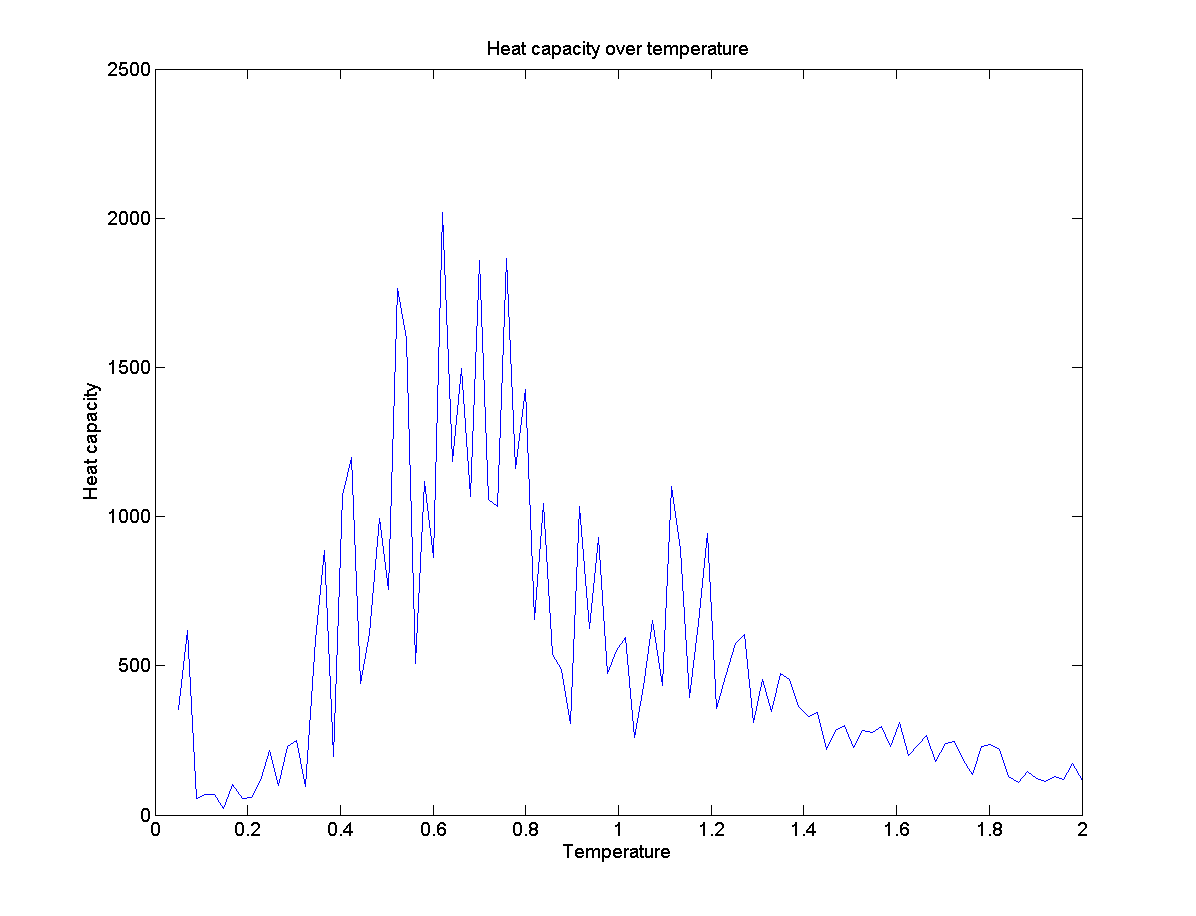
\includegraphics[width=\textwidth]{HoverT.png}
\caption{Heat capacity as a function of temperature}
\label{fig:HoverT}
\end{figure}
Using heat capacity, we can calculate the entropy of the system. This is done by using the matlab function Trapz, which is a numerical integration tool. This graph can be seen in figure \ref{fig:SoverT}:

\begin{figure}[h]
\centering
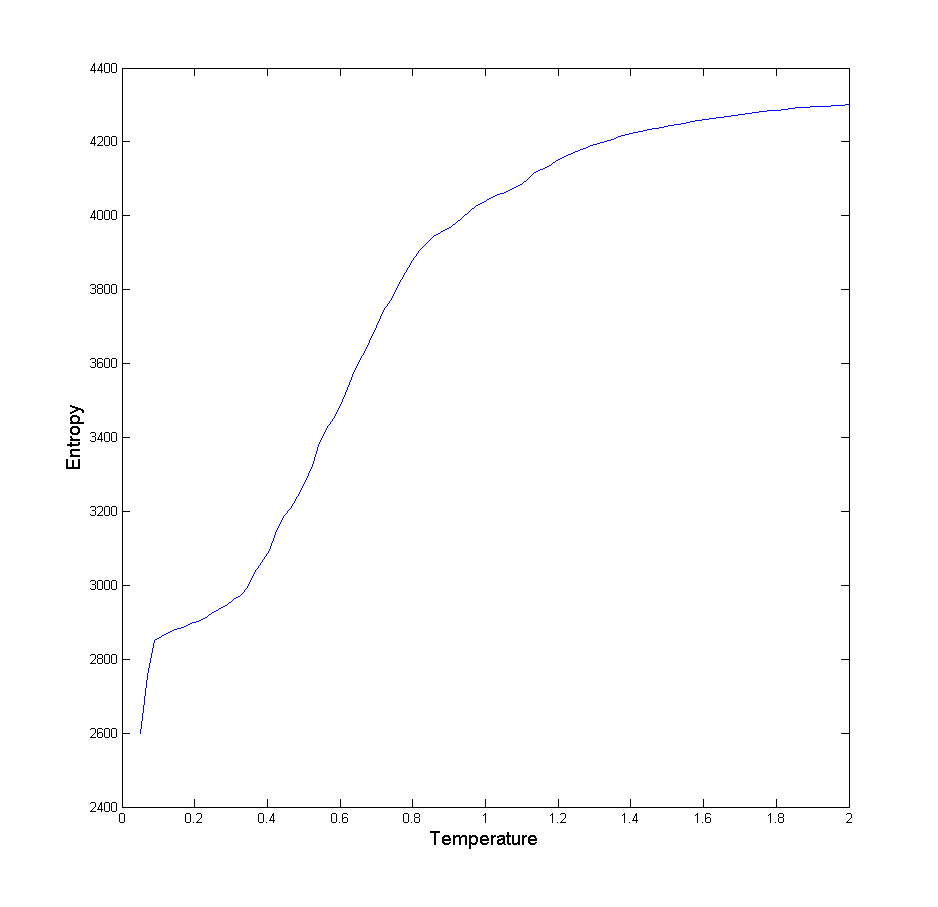
\includegraphics[width=\textwidth]{SoverT.png}
\caption{Entropy as a function of temperature}
\label{fig:SoverT}
\end{figure}
We use the found entropy to calculate the Helmholtz free energy, this is done by $F \equiv U-TS$. $U$ fluctuates greatly, we have fitted a logistic growth function upon the data and used that to calculate the Helmholtz free energy. This fit can be seen in figure \ref{fit}.  The entropy figure \ref{fig:FoverT} is shown:

\begin{figure}[h]
\centering
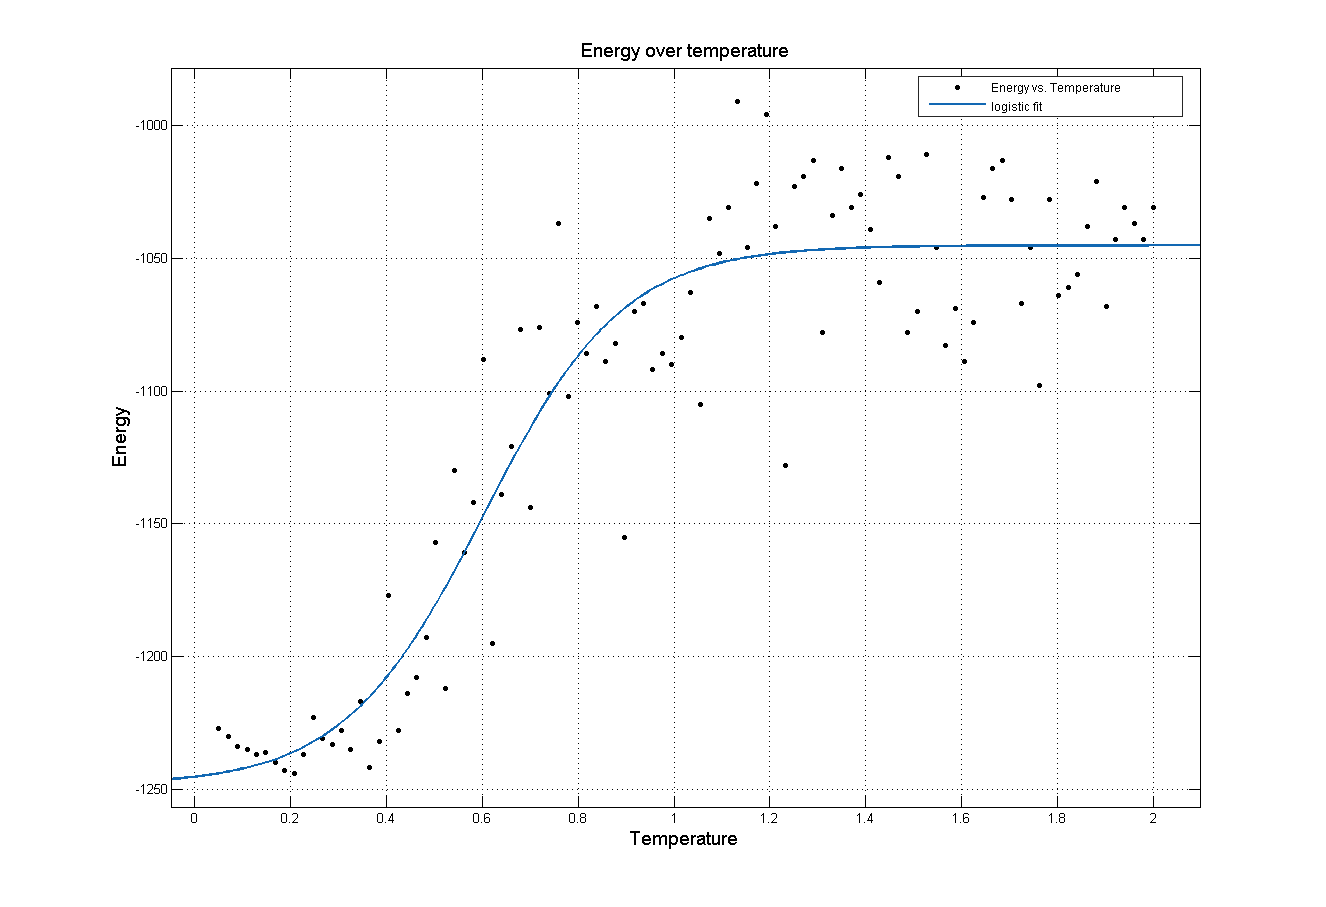
\includegraphics[width=\textwidth]{fit.png}
\caption{The logistic growth fit on the energy data}
\label{fit}
\end{figure}

\begin{figure}[h]
\centering
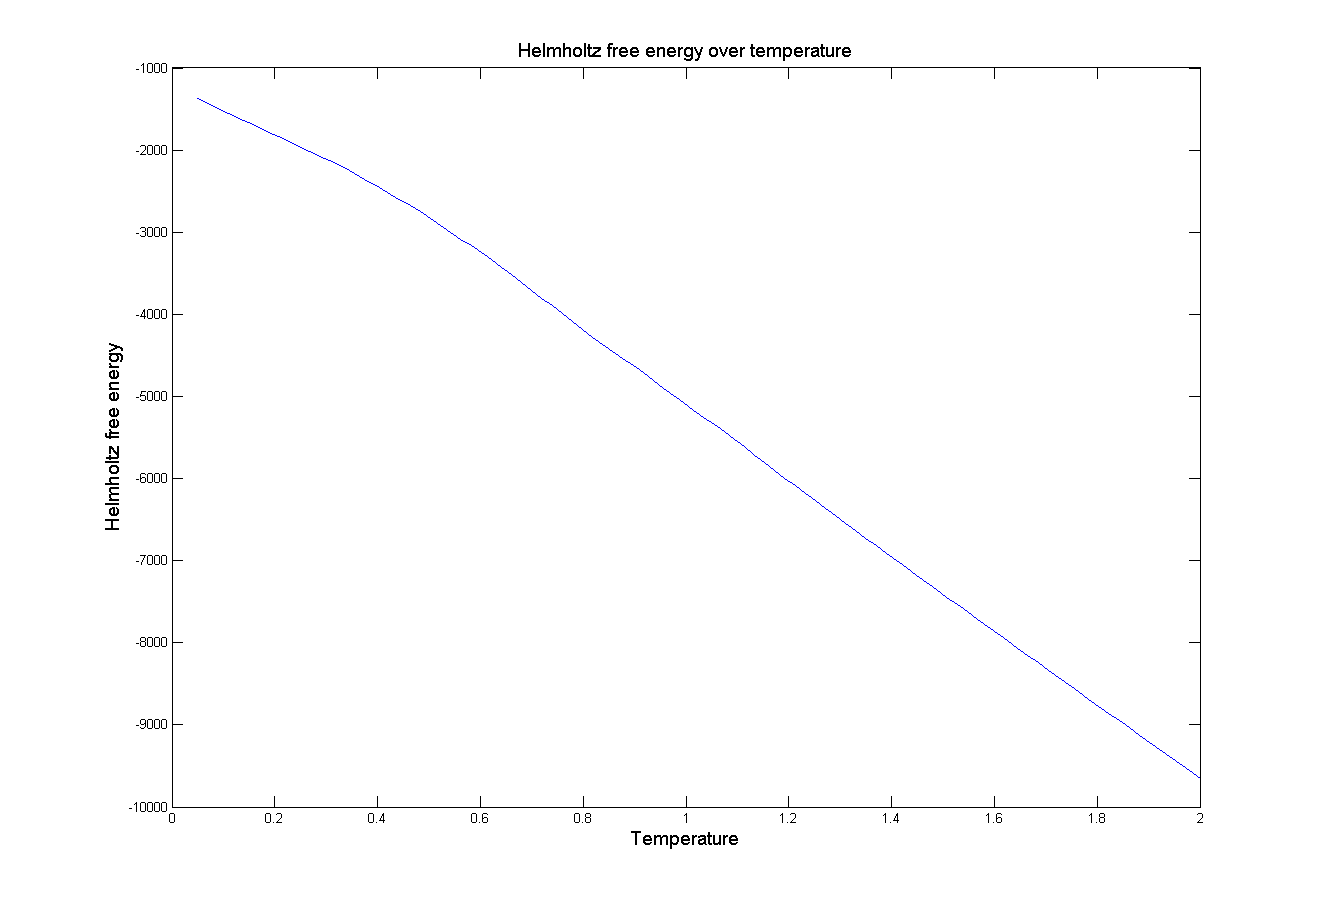
\includegraphics[width=\textwidth]{FoverT.png}
\caption{Helmholtz free energy as a function of temperature}
\label{fig:FoverT}
\end{figure}

Using the Helmholtz free energy, we calculate the chemical potential energy and then the Gibbs free energy. The Gibbs free energy for our mix can been seen in figure \ref{fig:GoverT}:

\begin{figure}[h]
\centering
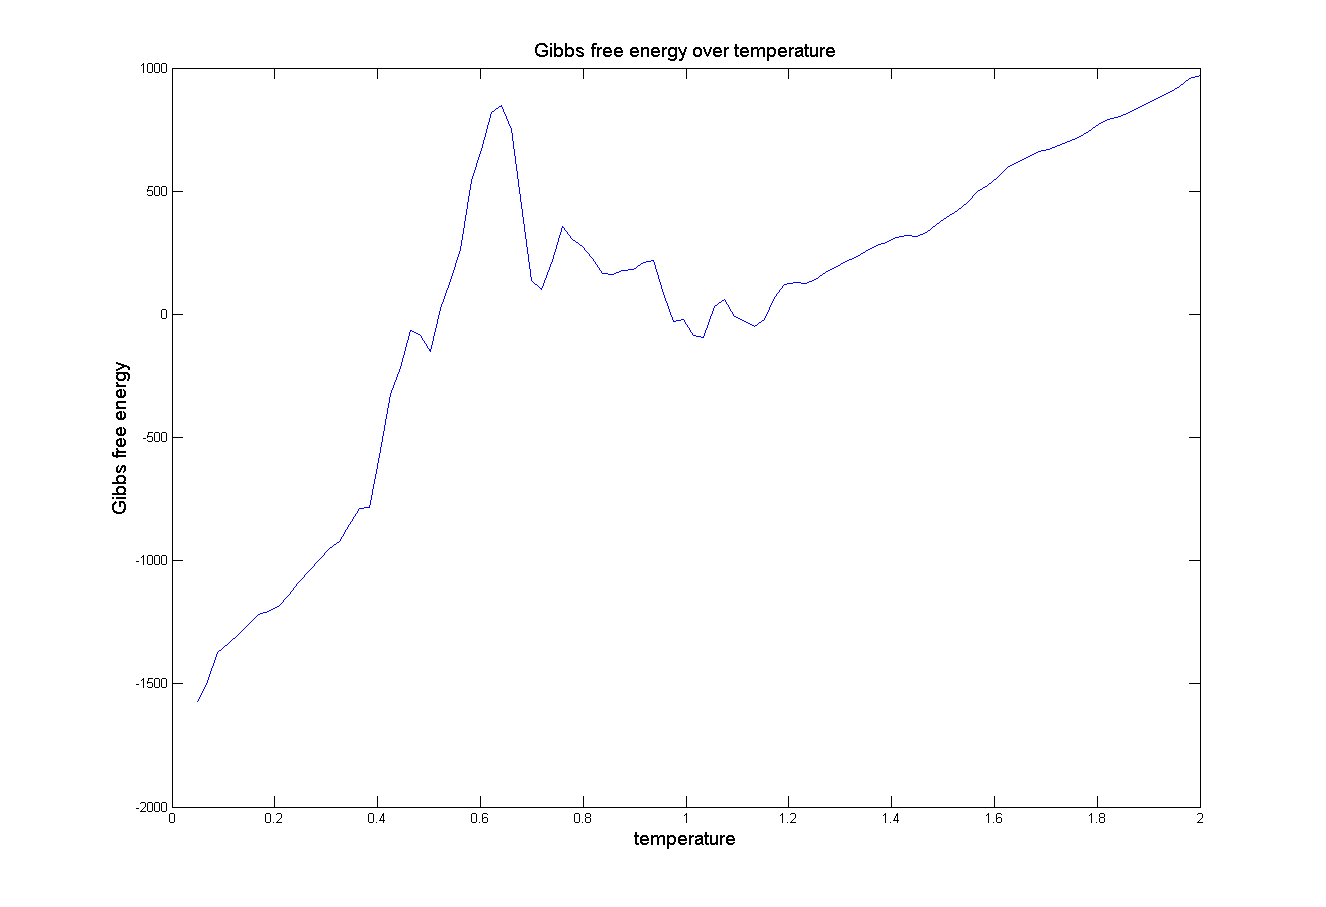
\includegraphics[width=\textwidth]{GoverT.png}
\caption{Gibbs free energy as a function of temperature}
\label{fig:GoverT}
\end{figure}

   

\chapter{Conclusion}
An ideal two dimension system of mixing of two types of particles can be simulated by the Monte Carlo Method and the theory of statistical mechanics and thermodynamics can be applied to analyse the system. If we had more time, we would work toward creating more Gibbs free energy curves and analysing the tendencies of the system.

\chapter{Matlab Code}
\lstinputlisting{mixing.m}
\lstinputlisting{genpopmix.m}
\lstinputlisting{energi.m}
\lstinputlisting{energy.m}
\lstinputlisting{entropi.m}


\end{document}